\documentclass[letterpaper,twocolumn,10pt]{article}

\usepackage{fullpage}
\usepackage{graphicx}
\usepackage{amsmath}
\usepackage{amssymb}
\usepackage{booktabs}
\usepackage{multirow}
\usepackage[hyphens]{url}
\usepackage[round]{natbib}
\usepackage{hyperref}
\usepackage{stfloats}
\usepackage{float}

\renewcommand*\ttdefault{lmvtt}
\newcommand{\dt}{\Delta t}
\newcommand{\train}{\mathrm{train}}
\newcommand{\test}{\mathrm{test}}
\newcommand{\argmax}{\operatornamewithlimits{argmax}}
\sloppy

\begin{document}

\title{Reproducing Programmatic Policy Generalization on Continuous-Force CartPole}
\date{}

\author{Jiawen Zhang\\
Independent Reproduction Study\\
{\tt Code and artifacts available in the accompanying repository}}

\maketitle

\begin{abstract}
Programmatic policies are designed to encode reusable control structure, while
neural policies often solve short training horizons without robustly
generalizing to longer test horizons.  We present a reproduction-oriented
engineering study of the CartPole benchmark from \emph{Synthesizing
Programmatic Policies that Inductively Generalize}.  We implement a
continuous-force CartPole environment, PyTorch PPO with feed-forward and LSTM
policies, and a compact two-mode programmatic state-machine learner.  The
implementation follows the paper's CartPole split: training uses a 5-second
horizon with pole length 0.5, and testing uses a 300-second horizon with pole
length 1.0.  Local diagnostic result claims are generated from repository
artifacts.
% Generated by scripts/make_paper_figures.py from CartPole result artifacts.
% Local diagnostic artifacts only; not a paper-scale reproduction of the 10^7-timestep, five-seed PPO/PPO-LSTM protocol.
In local diagnostics, feed-forward PPO reaches 100\% training success and obtains 0\% success on the full 300-second test horizon with mean test reward 910.6. The fixed programmatic state machine reaches 100\% training success, obtains 20\% full-horizon test success, and has mean test reward 6275.4.

We also document three implementation bugs that materially changed
reinforcement-learning behavior: missing 5-second episode truncation,
inconsistent continuous-action log probabilities after clipping, and recurrent
state mismatch in PPO-LSTM updates.
\end{abstract}

\footnotetext{Code and audit artifacts are in the accompanying repository.}

\section{Introduction}

Deep reinforcement-learning policies can be effective on the training
distribution while failing under longer horizons or shifted dynamics
\citep{packer2018generalization}.  The programmatic-policy hypothesis is that a
small controller with explicit modes and switches can encode reusable behavior
more directly than a monolithic neural network.  The original SPPIG paper
\citep{inala2020sppig} studies this hypothesis across several continuous
control tasks, including a CartPole setting where the train and test
distributions differ in both horizon and pole length.

This paper is a reproduction engineering study rather than a new algorithmic
claim.  We focus on one benchmark, continuous-force CartPole, and ask which
implementation details are necessary before neural and programmatic policies
can be compared fairly.  This framing is useful because reproduction failures
in reinforcement learning often come from small mismatches in horizon handling,
reward conventions, action distributions, or recurrent-state replay.

Our contributions are:
\begin{enumerate}
  \item \textbf{A faithful CartPole split.} We implement the CartPole row from
  the SPPIG benchmark table: one continuous action, four observations, training
  at 5 seconds with length 0.5, and testing at 300 seconds with length 1.0.
  \item \textbf{Executable PyTorch baselines.} We implement PPO with both
  feed-forward and LSTM actor-critic policies, generalized advantage
  estimation, vectorized rollouts, and best-checkpoint selection.
  \item \textbf{A compact programmatic controller.} We synthesize a two-mode
  constant-action state machine with an explicit switch over pole angle and
  angular velocity.
  \item \textbf{A debugging audit.} We identify and fix implementation errors
  that caused PPO to optimize the wrong objective or update recurrent policies
  under the wrong hidden state.
\end{enumerate}

\section{Benchmark Formulation}
\label{sec:benchmark}

The CartPole state is
\[
    x_t = (p_t, \dot p_t, \theta_t, \dot\theta_t),
\]
where $p_t$ is cart position, $\theta_t$ is pole angle, and the action
$a_t \in \mathbb{R}$ is a horizontal force clipped to $[-10, 10]$.  The
environment uses the standard CartPole reward convention: each simulated step
before truncation contributes one unit of survival reward.

\paragraph{Train/test split.}
The reproduction follows the paper's split:
\[
X_0^\train: T=5\mathrm{s}, \ell=0.5
\quad\quad
X_0^\test: T=300\mathrm{s}, \ell=1.0.
\]
With simulator step size $\dt = 0.02$, the training horizon is 250 steps and
the test horizon is 15,000 steps.  Success means surviving the entire relevant
horizon.

\paragraph{Policy objective.}
For a policy $\pi$, rollout reward is survival time up to the split horizon:
\[
    R(\pi) = \sum_{t=0}^{T/\dt - 1} \mathbf{1}\{\text{not failed at } t\}.
\]
Training optimizes the short-horizon distribution $X_0^\train$, while
generalization is evaluated on $X_0^\test$.

\section{Policy Classes}

\subsection{Feed-forward PPO}

The feed-forward PPO policy is a Gaussian actor-critic network.  Observations
are normalized by fixed CartPole scales and passed through two tanh hidden
layers.  The actor mean is squashed to the environment force range.  During
rollout collection, PPO stores the raw sampled action for log-probability
computation and clips only the force passed to the environment.  This avoids
mixing a clipped action with the probability density of a different raw sample.

\subsection{PPO-LSTM}

The recurrent baseline uses an observation encoder, an LSTM core, and actor and
critic heads.  The implementation stores the recurrent state at the start of
each rollout chunk and replays the same initial state during PPO updates.  This
is necessary because recomputing old action probabilities from a zero hidden
state changes the policy context used in the PPO ratio.

\subsection{Programmatic State Machine}

The programmatic learner constructs teacher traces and fits a two-mode
constant-action state machine in the CartPole grammar class.  The resulting
controller is:
% Generated by scripts/make_paper_figures.py from a PSM metrics artifact.
\[
  a(x_t) =
  \begin{cases}
    +10, & 10\theta_t + 1\dot{\theta}_t \ge 0,\\
    -10, & \text{otherwise}.
  \end{cases}
\]

This is intentionally compact: two constant actions and one interpretable
switching boundary.  It is not the full probabilistic adaptive-teaching
algorithm from \citet{inala2020sppig}.

\begin{figure*}[!t]
\centering
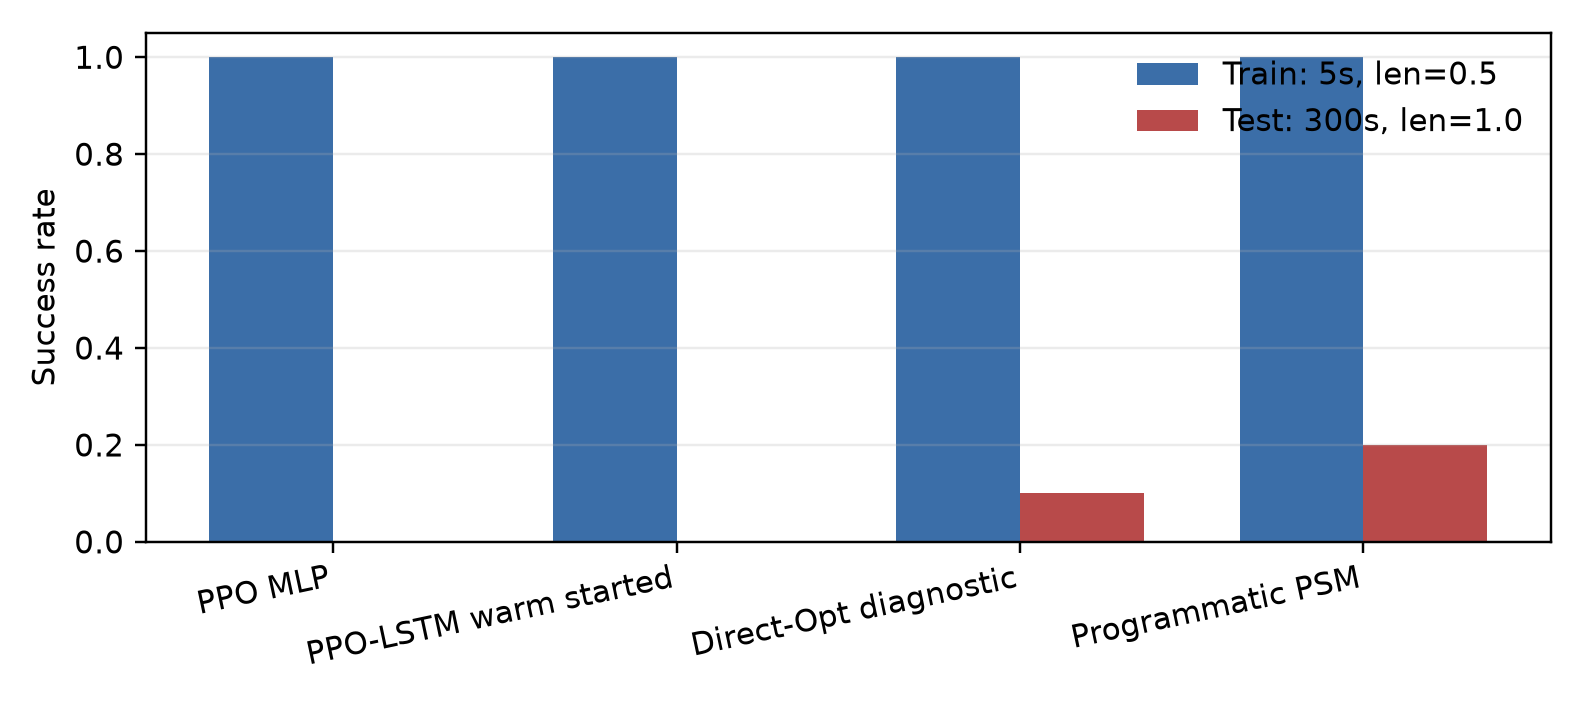
\includegraphics[width=0.31\textwidth]{figures/cartpole_success_rates.png}
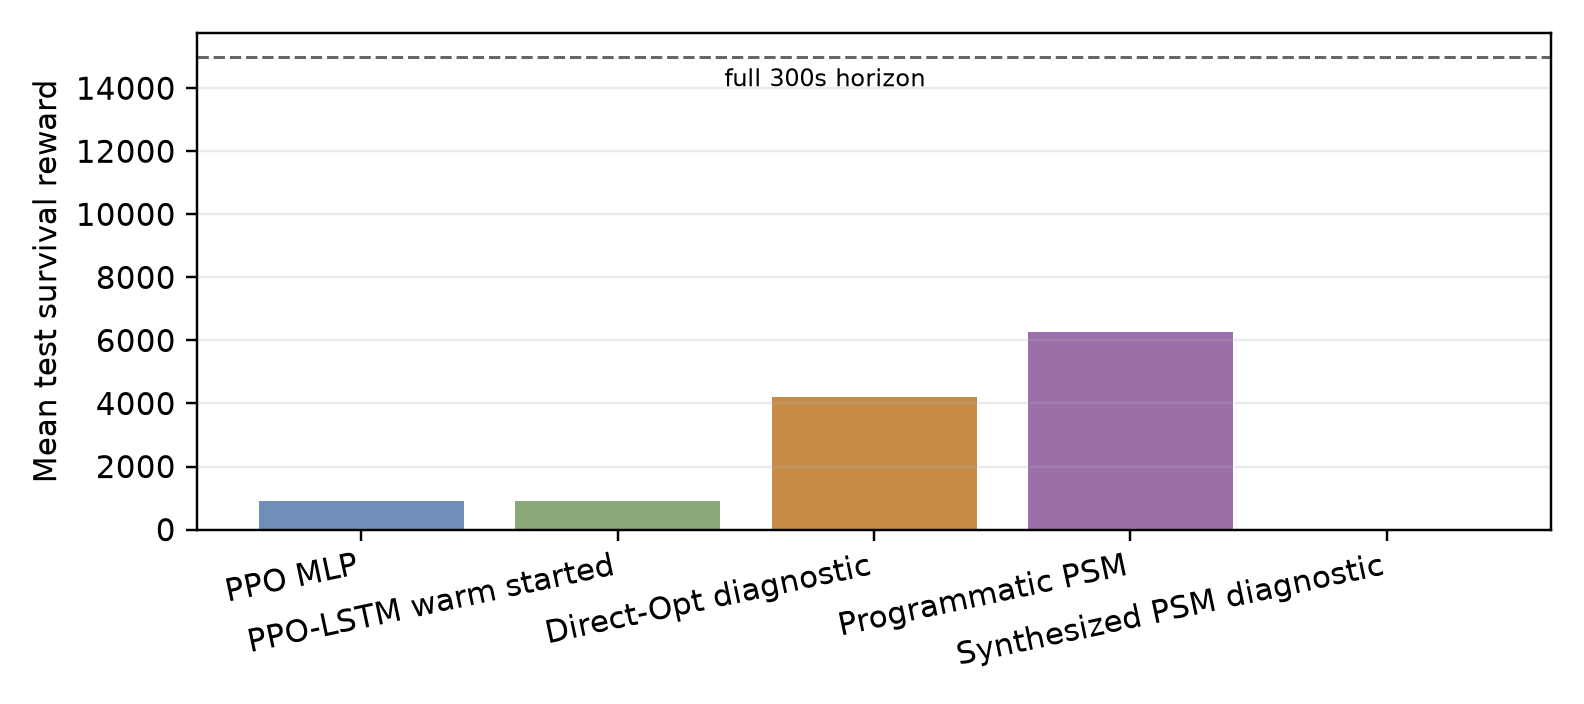
\includegraphics[width=0.31\textwidth]{figures/cartpole_test_survival_reward.png}
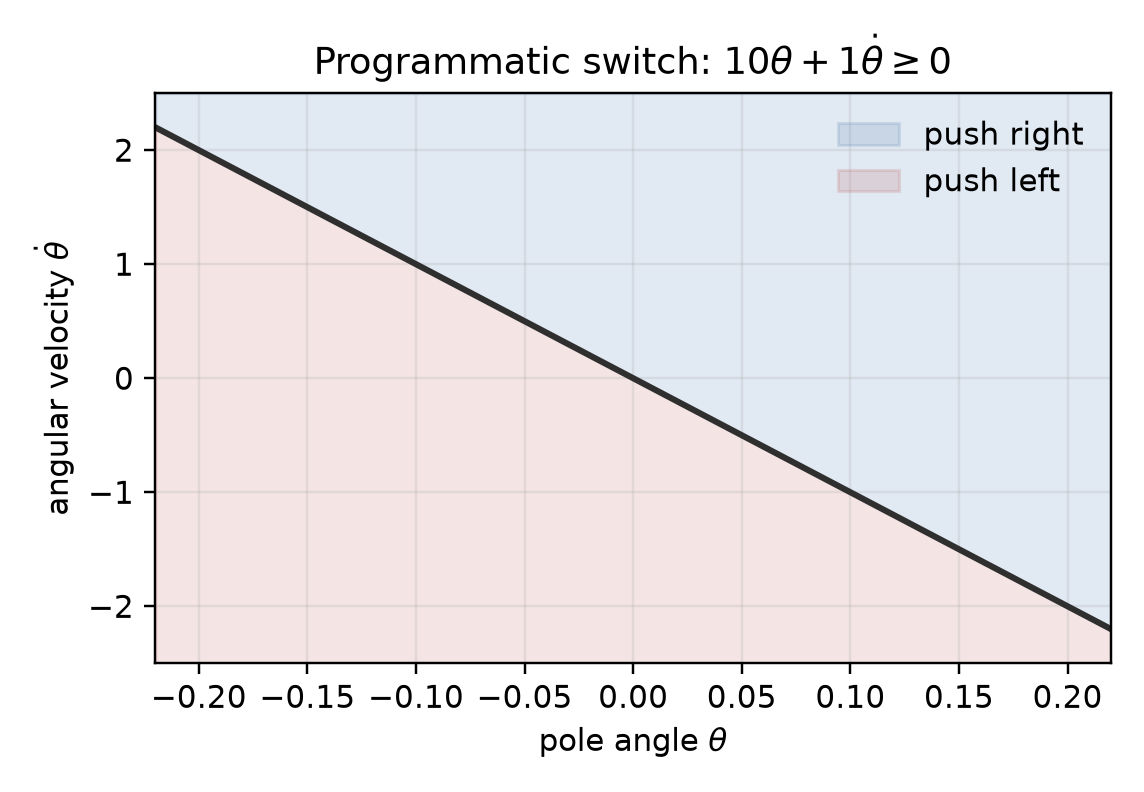
\includegraphics[width=0.31\textwidth]{figures/programmatic_switch_boundary.png}
\caption{Local CartPole reproduction diagnostics.  Left: train and full-horizon
test success rates.  Middle: mean survival reward on the 300-second test split.
Right: the learned programmatic switch boundary in $(\theta,\dot\theta)$ space.}
\label{fig:diagnostics}
\end{figure*}

\section{Implementation Audit}

Table~\ref{tab:params} summarizes the verified benchmark and diagnostic
settings.  The audit is part of the contribution because several seemingly
minor choices changed the outcome of PPO training.

\begin{table}[t]
\centering
\caption{Verified benchmark and local diagnostic settings.}
\label{tab:params}
\begin{tabular}{ll}
\toprule
Parameter & Value \\
\midrule
Observation dimension & 4 \\
Action dimension & 1 continuous force \\
Force range & $[-10, 10]$ \\
Simulator step $\dt$ & 0.02 \\
Train horizon & 5s = 250 steps \\
Train pole length & 0.5 \\
Test horizon & 300s = 15,000 steps \\
Test pole length & 1.0 \\
Programmatic modes & 2 \\
Action grammar & Constant \\
Switch grammar & Boolean tree, depth 2 \\
Diagnostic rollouts & 20 \\
\bottomrule
\end{tabular}
\end{table}

\paragraph{Horizon truncation.}
The most important bug was training PPO without truncating episodes at the
paper's 5-second training horizon.  Resetting only after physical failure
turned the baseline into an indefinite survival task.  After fixing truncation,
feed-forward PPO reached 100\% training success in local diagnostics.

\paragraph{Continuous actions.}
For continuous-action PPO, clipping sampled actions before both environment
execution and log-probability storage creates a mismatch.  The implementation
now stores raw sampled actions for PPO ratios and clips only the environment
force.

\paragraph{Recurrent state.}
For PPO-LSTM, rollout collection can begin in the middle of an episode with a
nonzero hidden state.  Updating from a zero hidden state computes likelihoods
under a different recurrent context.  The implementation now stores and reuses
the rollout's initial recurrent state.

\section{Experimental Results}

Table~\ref{tab:results} reports the verified local comparison.  The
feed-forward PPO and programmatic policies both solve the 250-step training
split.  On the full 15,000-step test split, the programmatic controller
survives much longer and has nonzero full-horizon success.

\begin{table}[t]
\centering
\caption{Local diagnostic evaluation generated from repository result
artifacts.  Test success uses the full
300-second horizon.}
\label{tab:results}
% Generated by scripts/make_paper_figures.py from CartPole result artifacts.
\begin{tabular}{lrrrr}
\toprule
Policy & Train succ. & Test succ. & Train rew. & Test rew. \\
\midrule
PPO MLP & 1.00 & 0.00 & 250.0 & 910.6 \\
PPO-LSTM warm started & 1.00 & 0.00 & 250.0 & 912.2 \\
Direct-Opt diagnostic & 1.00 & 0.10 & 250.0 & 4220.1 \\
Programmatic PSM & 1.00 & 0.20 & 250.0 & 6275.4 \\
\bottomrule
\end{tabular}

\end{table}

\paragraph{PPO-LSTM status.}
Pure PPO-LSTM is implemented and executable, but did not solve the training
split within the local diagnostic budget.  A supervised warm start from the
programmatic controller followed by PPO fine-tuning does solve the training
split, showing that the recurrent architecture can represent a working policy.
We therefore report warm-started PPO-LSTM separately and do not treat it as the
paper's pure PPO-LSTM baseline.

\section{Related Work}

CartPole is a classic benchmark for adaptive control \citep{barto1983cartpole}.
PPO \citep{schulman2017ppo} and generalized advantage estimation
\citep{schulman2015gae} are standard components of deep reinforcement-learning
baselines, and the original SPPIG comparison used OpenAI Baselines PPO2
\citep{baselines}.  Programmatic policy learning has also been explored as a
path toward interpretable and generalizable controllers
\citep{trivedi2021programs}.  This work is closest to a reproduction audit of
the CartPole component of \citet{inala2020sppig}.

\section{Limitations}

This paper should not be read as a full reproduction of SPPIG.  The
programmatic learner here is a compact trace-based reconstruction, not the full
probabilistic adaptive-teaching and EM-style student algorithm.  The PPO
diagnostics are local runs, not the paper's $10^7$-timestep, five-seed,
hyperparameter-search protocol.  The extracted PDF text did not expose the
exact CartPole bar values from the original result figure or the exact
CartPole state-machine formula from the appendix figure, so those details
still require manual figure inspection.

\section{Reproducibility}

The repository includes tests, result tables, and command-line runners.  The
main verification command is:
\begin{verbatim}
python -m unittest discover -s tests
\end{verbatim}
The main experiment commands are:
\begin{verbatim}
python src/train_cartpole_psm.py --eval-rollouts 20 \
  --test-max-steps 15000
python src/train_cartpole_ppo.py --policy mlp \
  --timesteps 131072 --rollout-steps 128 \
  --num-envs 8 --eval-interval 16384 --verbose
\end{verbatim}
The paper-fidelity audit is maintained in
\texttt{docs/cartpole\_paper\_audit.md}.

\section{Discussion and Future Work}

The main lesson is that programmatic-policy comparisons are sensitive to
baseline implementation details.  Missing horizon truncation made PPO appear
much weaker because it optimized a different task.  After the audit,
feed-forward PPO solved the short training horizon, but still failed the full
300-second generalization test.  The programmatic state machine generalized
better in survival time because its switching boundary encodes a repeatable
balancing rule rather than a short-horizon neural behavior.

Before a strong arXiv submission, future work should run the paper-scale PPO
protocol: five seeds, hyperparameter search, and $10^7$ timesteps for both PPO
and PPO-LSTM.  The programmatic side should also be upgraded from the compact
trace-based learner to the full probabilistic adaptive-teaching algorithm if
exact algorithmic fidelity is required.

\section{Conclusion}

This reproduction study implements continuous-force CartPole, PPO, PPO-LSTM,
and a compact programmatic state machine under the SPPIG train/test split.  The
result supports the qualitative claim that explicit programmatic structure can
improve long-horizon generalization, while also showing that careful
reinforcement-learning engineering is necessary before such comparisons are
credible.

\section*{Acknowledgments}

ChatGPT/Codex was used as an engineering assistant for code implementation,
debugging, and draft editing.  All claims in this draft should be verified
against the accompanying code and audit logs before submission.

\bibliographystyle{apalike}
\bibliography{project}

\end{document}
